% TeX encoding = utf8
% TeX spellcheck = pl_PL 
\documentclass[a4paper,titlepage,11pt,twosides,floatssmall]{mwrep}
\usepackage[left=2.5cm,right=2.5cm,top=2.5cm,bottom=2.5cm]{geometry}
\usepackage[OT1]{fontenc}
\usepackage{polski}
\usepackage{amsmath}
\usepackage{amsfonts}
\usepackage{amssymb}
\usepackage{graphicx}
\usepackage{url}
\usepackage{tikz}
\usetikzlibrary{arrows,calc,decorations.markings,math,arrows.meta}
\usepackage{rotating}
\usepackage[percent]{overpic}
\usepackage[utf8]{inputenc}
\usepackage{xcolor}
\usepackage{pgfplots}
\usetikzlibrary{pgfplots.groupplots}
\usepackage{listings}
\usepackage{matlab-prettifier}
\usepackage{siunitx}
\usepackage[section]{placeins}
\definecolor{szary}{rgb}{0.95,0.95,0.95}
\SendSettingsToPgf
\sisetup{detect-weight,exponent-product=\cdot,output-decimal-marker={,},per-mode=symbol,binary-units=true,range-phrase={-},range-units=single}

%konfiguracje pakietu listings
\lstset{
	backgroundcolor=\color{szary},
	frame=single,
	breaklines=true,
}
\lstdefinestyle{customlatex}{
	basicstyle=\footnotesize\ttfamily,
	%basicstyle=\small\ttfamily,
}
\lstdefinestyle{customc}{
	breaklines=true,
	frame=tb,
	language=C,
	xleftmargin=0pt,
	showstringspaces=false,
	basicstyle=\small\ttfamily,
	keywordstyle=\bfseries\color{green!40!black},
	commentstyle=\itshape\color{purple!40!black},
	identifierstyle=\color{blue},
	stringstyle=\color{orange},
}
\lstdefinestyle{custommatlab}{
	captionpos=t,
	breaklines=true,
	frame=tb,
	xleftmargin=0pt,
	language=matlab,
	showstringspaces=false,
	%basicstyle=\footnotesize\ttfamily,
	basicstyle=\scriptsize\ttfamily,
	keywordstyle=\bfseries\color{green!40!black},
	commentstyle=\itshape\color{purple!40!black},
	identifierstyle=\color{blue},
	stringstyle=\color{orange},
}

%wymiar tekstu (bez żywej paginy)
\textwidth 160mm \textheight 247mm

%ustawienia pakietu pgfplots
\pgfplotsset{
	tick label style={font=\scriptsize},
	label style={font=\small},
	legend style={font=\small},
	title style={font=\small}
}

\def\figurename{Rys.}
\def\tablename{Tab.}

%konfiguracja liczby pływających elementów
\setcounter{topnumber}{0}%2
\setcounter{bottomnumber}{3}%1
\setcounter{totalnumber}{5}%3
\renewcommand{\textfraction}{0.01}%0.2
\renewcommand{\topfraction}{0.95}%0.7
\renewcommand{\bottomfraction}{0.95}%0.3
\renewcommand{\floatpagefraction}{0.35}%0.5

\begin{document}
	
	\begin{titlepage}
		\begin{center}
			\Huge{\textsc{Sprawozdanie z trzeciej części projektu z przedmiotu \\,,Technika Automatyzacji Procesów''}} \\
			[15cm]
			\Large{Numer zadania: 3 \\Wykonawcy:}\\
			\Large{Dawidiuk Marek \\ Giełdowski Daniel \\ Kłos Maciej \\ Taras Sylwia}
		\end{center}
	\end{titlepage}
	
	\tableofcontents
	\newpage
	\chapter{Opis otrzymanego modelu}

W ramach tego projektu korzystaliśmy z modelu obiektu znanego jako reaktor przepływowy. Obiekt składa się z pojemnika wypełnionego cieczą z rozpuszczoną nieokreśloną substancją. Do pojemnika wpływa strumieniem $F_{in}$ ciecz o określonej temperaturze $T_{in}$ oraz stężeniu rozpuszczonej substancji $C_{Ain}$. W pojemniku jest określona ilość cieczy $V$ w określonej temperaturze $T$. Ciecz z pojemnika wypływa strumieniem $F$, zawierając stężenie $C_A$ rozpuszczonej substancji. Dodatkowo przez pojemnik przeprowadzona jest rura odpowiedzialna za chłodzenie bądź podgrzewanie, którą strumieniem $F_C$ płynie ciecz o temperaturze wejściowej $T_{Cin}$. Obiekt opisany jest następującymi równaniami:
\begin{equation}
	\left\{
	\begin{tabular}{l}
	$V \cdot \frac{dC_A}{dt}=F_{in} \cdot C_{Ain}-F \cdot C_A-V \cdot k_0 \cdot e^{-\frac{E}{R \cdot T}} \cdot C_A$\\
	$V \cdot \rho \cdot c_p \cdot \frac{dT}{dt}=F_{in} \cdot \rho \cdot c_p \cdot T_{in}-F \cdot \rho \cdot c_p \cdot T+V \cdot h \cdot k_0 \cdot e^{-\frac{E}{R \cdot T}} \cdot C_A - \frac{a \cdot (F_C)^{b+1}}{F_C+\frac{a \cdot (F_C)^b}{2 \cdot \rho_c \cdot c_{pc}}} \cdot (T-T_{Cin})$
	\end{tabular}
	\right.
\end{equation}
W równaniach występują stałe o podanych wartościach:\\
\begin{itemize}
	\item $\rho=\rho_c=10^6\frac{g}{m^3}$
	\item $c_p=c_{pc} = 1 \frac{cal}{g\cdot K}$
	\item $k_0 = 10^{10} \frac{1}{min}$
	\item $\frac{E}{R} = 8330,1 \frac{1}{K}$
	\item $h = 130\cdot 10^6 \frac{cal}{kmol}$
	\item $a = 1,678\cdot 10^6\frac{cal}{K\cdot m^3}$
	\item $b = 0,5$
\end{itemize}
Otrzymaliśmy także dane odnośnie wartości zmiennych modelu w zadanym punkcie pracy układu:\\
\begin{itemize}
	\item $V=1m^3$
	\item $F_{in} = F = 1 \frac{m^3}{min}$
	\item $C_{Ain} = 2 \frac{kmol}{m^3}$
	\item $F_C = 15 \frac{m^3}{min}$
	\item $T_{in} = 323K$
	\item $T_{Cin} = 365K$
	\item $C_A = 0,26\frac{kmol}{m^3}$
	\item $T = 393,9K$
\end{itemize}
W ramach zadania zmienne te podzielone zostały na 4 grupy:\\
\begin{itemize}
	\item stałe - $V,F,F_{in}$
	\item regulowane - $C_A,T$
	\item sterujące - $C_{Ain},F_C$
	\item zakłócenia - $T_{in},T_{Cin}$
\end{itemize}
Po zastąpieniu stałych w równaniach liczbami, otrzymywany jest następujący układ równań:\\
\begin{equation}
	\left\{
	\begin{tabular}{l}
	$\frac{dC_A}{dt} = C_{Ain} - C_A - 10^{10}\cdot e^{-\frac{8330,1}{T}}\cdot C_A$\\
	$\frac{dT}{dt} = T_{in} - T + 130\cdot 10^{10}\cdot e^{-\frac{8330,1}{T}}\cdot C_A-\frac{1,678\cdot (F_C)^{1,5}}{F_C+0,839\cdot (F_C)^{0,5}}(T-T_{Cin})$
	\end{tabular}
	\right.
\end{equation}
Ostatnią rzeczą jaka musiała zostać wzięta pod uwagę było dokładniejsze określenie wartości wyjść w punkcie pracy, ponieważ te podane w zadaniu były przybliżone. Proces ten został wykonany w pierwszej części projektu, a wartości wyjść wyniosły w przybliżeniu $C_A = 0,2646$ oraz $T = 393,9531$.

	\chapter{Implementacja obiektu}

Pierwszym zadaniem do wykonania podczas tej części projektu była implementacja zadanego obiektu w środowisku OVATION. Zanim jednak przystąpiliśmy do implementacji należało przekształcić model z równań ciągłych na dyskretne. Zgodnie z instrukcją podaną przez prowadzącego zostało to wykonane poprzez proste podstawienie, w którym k to numer kroku modelu, a $T_S$ oznacza czas próbkowania:

\begin{equation}
\left\{
\begin{tabular}{l}
$\frac{dC_A}{dt} = \frac{C_{A_{k+1}}-C_{A_k}}{T_s}$\\
$\frac{dT}{dt} = \frac{T_{k+1}-T_k}{T_s}$
\end{tabular}
\right.
\end{equation}

Jako czas próbkowania przyjęliśmy 1 sekundę. Ponieważ jednak nasz obiekt posługuje się nominalnie minutami wartość $T_s$ wyniosła 1/60. Ostatecznie więc do implementacji otrzymaliśmy następujące równania:

\begin{equation}
\left\{
\begin{tabular}{l}
$C_{A_{k+1}} = (C_{Ain_k} - C_{A_k} - 10^{10}\cdot e^{-\frac{8330,1}{T_k}}\cdot C_{A_k})/60+C_{A_k}$\\
$T_{k+1} =( T_{in_k} - T_k + 130\cdot 10^{10}\cdot e^{-\frac{8330,1}{T_k}}\cdot C_{A_k}-\frac{1,678\cdot (F_{C_k})^{1,5}}{F_{C_k}+0,839\cdot (F_{C_k})^{0,5}}(T_k-T_{Cin_k}))/60+T_k$
\end{tabular}
\right.
\end{equation}

Mając tak przygotowane wzory przystąpiliśmy do implementacji, którą rozpoczęliśmy od utworzenia odpowiednich punktów wejściowych (4 punkty: 2 dla sterowania i 2 dla zakłóceń) i wyjściowych (2 punkty). Utworzone zostały punkty o następujących nazwach(zgodnie z przyjętą konwencją nazewnictwa obejmującą numer grupy):
\begin{itemize}
	\item 3\_CAIN\_IN
	\item 3\_FC\_IN
	\item 3\_TIN\_IN
	\item 3\_TCIN\_IN
	\item 3\_CA\_OUT
	\item 3\_T\_OUT
\end{itemize}
Punkty odpowiadające sterowaniom oraz wyjściom obiektu zostały następnie przypisane odpowiednio do bloków wejść i wyjść wewnątrz arkusza projektowego. Punkty zakłóceń zadane zostały poprzez użycie bloków AVALGEN. Dodatkowo sterowania podłączone zostały poprzez blok TRANSFER sterowany sygnałem binarnym. Blok ten określa, czy w danej chwili regulator pracuje w trybie ręcznym czy też automatycznym.

Po umieszczeniu wejść oraz wyjść modelu na arkuszu nadeszła pora na implementację samego obiektu. W tym celu wykorzystaliśmy bloki CALCBLOCK umożliwiające dokonywanie obliczeń z wykorzystaniem do 18 zmiennych wejściowych, z których to wejść nasz model wykorzystywał jedynie 6. Dla każdego użytego bloku, jako wejścia od IN1 do IN6 posłużyły nam kolejno: $C_{Ain}, F_C, T_{in}, T_{Cin}, C_A$ oraz $T$. Implementacja pierwszego równania obyła się bez przeszkód. Jest ona przedstawiona na poniższym rysunku.

\begin{figure}[h!]
	\centering
	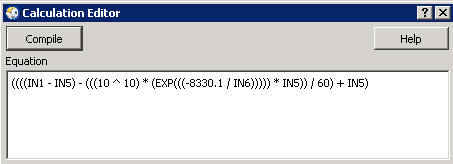
\includegraphics[width=.5\linewidth]{img/CALCBLOCK1.png}
	\label{ch1:calc1}
	\caption{Formuła pierwszego równania modelu wewnątrz CALCBLOCK}
\end{figure}

Niewielki problem wystąpił podczas implementacji równania drugiego wyjścia modelu. Ze względu na ograniczenie nałożone na ilość znaków mogących się znaleźć wewnątrz formuły bloku CALCBLOK, działanie to musiało być przez nas podzielone na dwa bloki. W pierwszym z nich umieszczony został fragment: $T_{in_k} - T_k + 130\cdot 10^{10}\cdot e^{-\frac{8330,1}{T_k}}\cdot C_{A_k}$. Pozostałą część równania umieściliśmy w drugim. W celu wyraźnego odgraniczenia wyjścia pierwszego bloku od zmiennych procesu, zostało one wprowadzone do drugiego bloku jako IN18. Obydwa bloki zostały także odpowiednio połączone, tak aby kalkulacje w bloku drugim zachodziły zawsze po kalkulacjach bloku pierwszego, gdyż wykorzystujemy jego wyliczoną wartość. Zawartość obydwu bloków przedstawiona została na rysunkach poniżej.

\begin{figure}[h!]
	\centering
	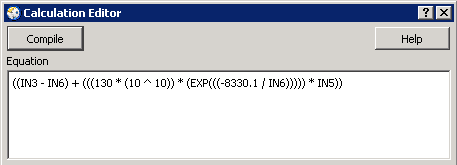
\includegraphics[width=.5\linewidth]{img/CALCBLOCK2.png}
	\label{ch1:calc2}
	\caption{Formuła wewnątrz pierwszego bloku CALCBLOCK dla drugiego równania modelu}
\end{figure}

\begin{figure}[h!]
	\centering
	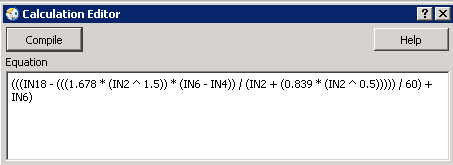
\includegraphics[width=.5\linewidth]{img/CALCBLOCK3.png}
	\label{ch1:calc3}
	\caption{Formuła wewnątrz drugiego bloku CALCBLOCK dla drugiego równania modelu}
\end{figure}

Po odpowiednim połączeniu wszystkich elementów otrzymaliśmy działający model zadanego dla nas obiektu. W celu jego przetestowania wykonaliśmy skok sterowania $C_{Ain}$ do wartości 1,6. Obiekt zachował się zgodnie z oczekiwaniami, a wartości wyjścia zbiegły do spodziewanych. Wynik zachowaliśmy w pliku csv, do późniejszego rysowania wykresu. Poniżej zamieszczamy wykresy otrzymane w wyniku tej symulacji.

\begin{figure}[h!]
	\centering
	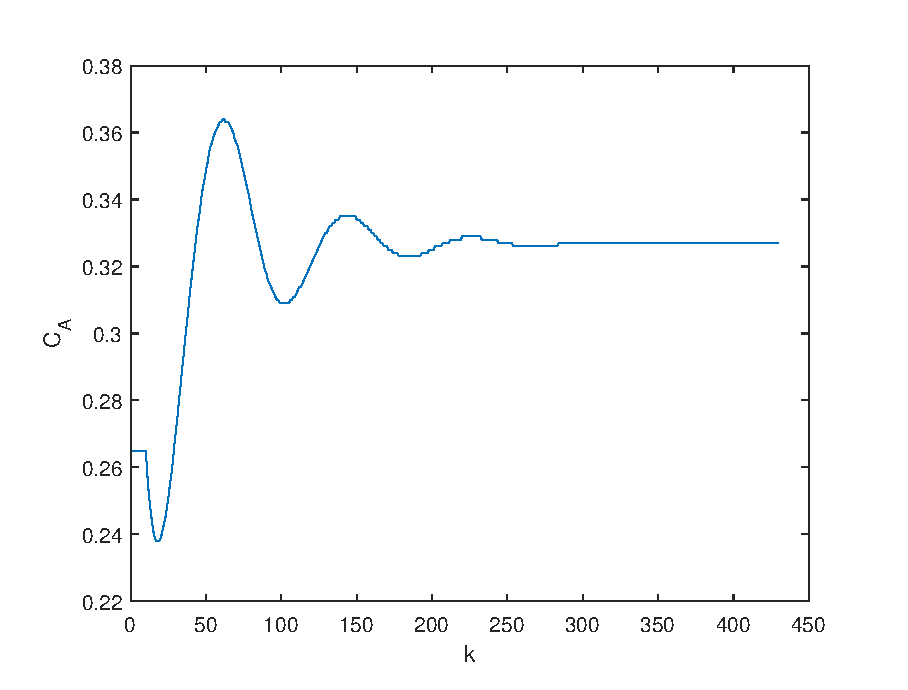
\includegraphics[width=.8\linewidth]{img/model1.eps}
	\label{ch1:model1}
	\caption{Wyjście $C_A$ modelu po skoku sterowania $C_{Ain}$ do 1,6}
\end{figure}

\begin{figure}[h!]
\centering
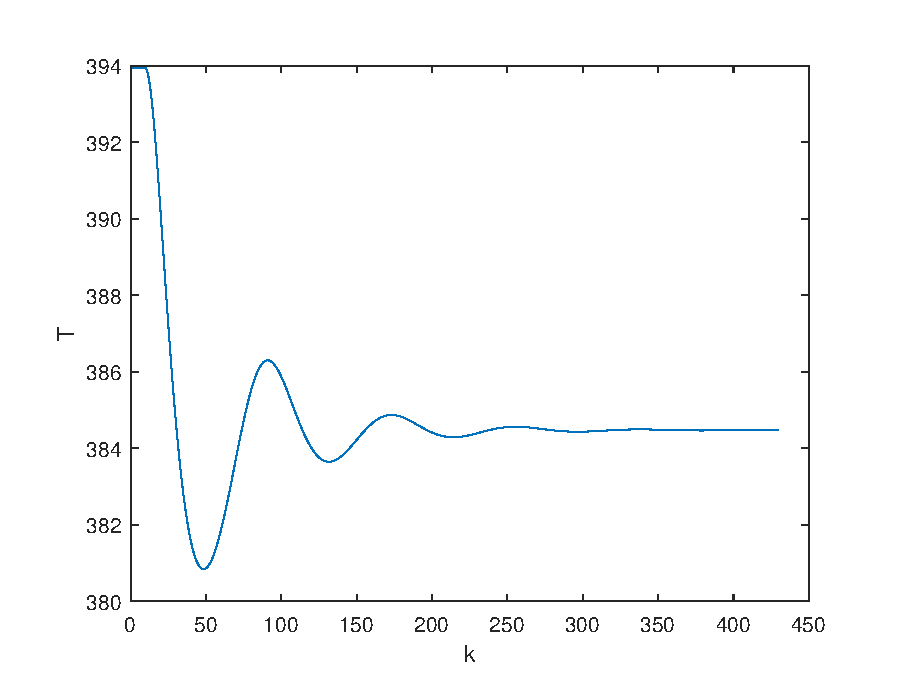
\includegraphics[width=.8\linewidth]{img/model2.eps}
\label{ch1:model2}
\caption{Wyjście $T$ modelu po skoku sterowania $C_{Ain}$ do 1,6}
\end{figure}

\begin{figure}[h!]
	\centering
	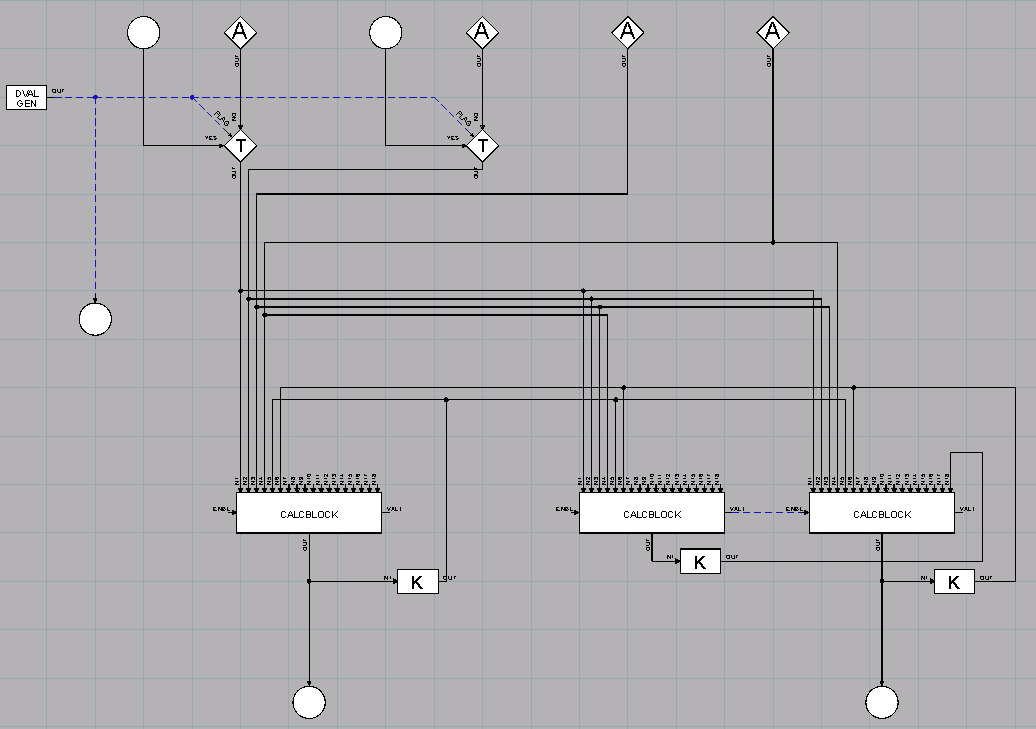
\includegraphics[width=\linewidth]{img/MODEL.png}
	\label{ch1:model}
	\caption{Model obiektu wykonany w programie OVATION}
\end{figure}

	\chapter{Regulator obiektu}
Drugim zadaniem wchodzącym w skład tej części projektu była implementacja działającego regulatora PID. Miał być to regulator równoległy bez odsprzęgania, innymi słowy składał się on z dwóch regulatorów PID nie ingerujących wzajemnie w swoje działanie. Każdy z nich otrzymywał na wejście uchyb jednego z wyjść i generował odpowiednie sterowanie. Wyjścia i wejścia zostały przez nas sparowane w następujący sposób: $C_A$ z $F_C$ oraz $T$ z $C_{Ain}$.
Decyzja ta została podyktowana charakterystyką działania obiektu określoną w pierwszej części projektu, według której zwiększenie sterowania $C_{Ain}$ powodowało spadek wartości wyjścia $C_A$, a zwiększenie $T$. Reakcja dla drugiego wyjścia była odwrotna.

Mając określone wejścia i wyjścia regulatorów mogliśmy przystąpić do implementacji w programie OVATION. Zgodnie z instrukcją prowadzącego posłużyliśmy się w tym celu blokiem regulatora PID obecnym w systemie. Dodatkowo skorzystaliśmy z przełącznika binarnego używanego w arkuszu modelu obiektu służącego do przełączania trybów sterowania: manualnego i regulowanego. W trybie manualnym regulatory zostają odcięte, a podawany na nie uchyb jest zerowany.

\begin{figure}[h!]
	\centering
	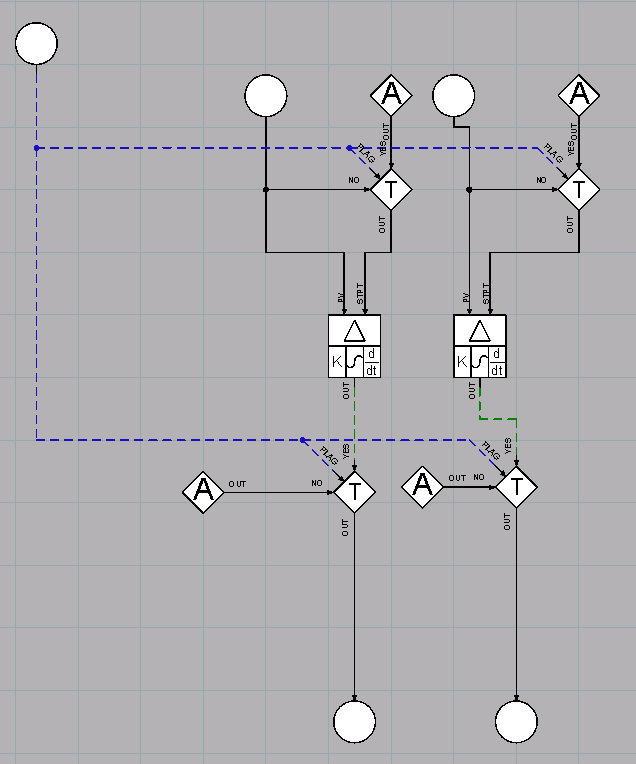
\includegraphics[width=.6\linewidth]{img/PID.png}
	\label{ch2:regulator}
	\caption{Model regulatora wykonany w programie OVATION}
\end{figure}
\newpage
Blok PID zawierał cztery parametry, które należało odpowiednio dobrać w celu osiągnięcia optymalnej regulacji. Ze względu na fakt, że strojenie regulatorów bezpośrednio na zaimplementowanym obiekcie mogłoby zająć więcej czasu niż mieliśmy, zdecydowaliśmy się dobrać nastawy z użyciem modelu wykonanego w programie Matlab i klasy regulatora, udostępnionej przez prowadzącego, bliźniaczo podobnej w działaniu do bloku obecnego w OVATION. Po uzyskaniu zadowalających wyników, przygotowane nastawy regulatorów przeniesione zostały do symulatora OVATION. Ze względu na fakt, że Matlab oraz OVATION używają innych rozmiarów zmiennych liczbowych, działanie symulacji nie było całkowicie identyczne z danymi uzyskanymi w programie Matlab. Z tego powodu nastawy regulatorów zostały przez nas dostrojone na podstawie wyników działania symulacji. Poniżej zamieszczamy tabelę z ostatecznymi parametrami obydwu regulatorów, uznanymi przez nas za optymalne.

\begin{table}[h!]
	\centering
	\begin{tabular}{|c|c|c|c|c|c|}
		\hline
		Zmienna regulowana&Wyjście&K&Ti&Kd&Td\\\hline
		$C_A$&$F_C$&10&0,55&80&10\\\hline
		$T$&$C_{Ain}$&0,002&600&0,2&1,8\\\hline
	\end{tabular}
\label{tab:pid}
\caption{Nastawy regulatorów PID}
\end{table}

Na koniec pozostało jeszcze zadanie udokumentowania działania zaimplementowanego przez nas układu regulacji. Poniżej przedstawiamy wyniki działania regulatorów w formie wykresów.

\begin{figure}[h!]
	\centering
	\includegraphics[width=.8\linewidth]{img/pid.eps}
	\label{ch2:pid}
	\caption{Działanie regulatora PID regulującego wyjście $C_A$}
\end{figure}

	
\end{document}